% !TEX root = IBL-InsolvabilityOfQuintic.tex
\chapter{Rings}
\label{chapter:Rings}
\thispagestyle{empty}
Our overarching goal, laid out in Chapter~\ref{chapter:PolyEquations}, is to show that there are quintic polynomials whose roots are \emph{not} expressible in terms of its coefficients using just the operations of addition, subtraction, multiplication, division, and the extraction of roots (thus implying that there is no ``quintic formula'' that is analogous to the quadratic formula). We decided that we would say that such polynomials are \emph{not} solvable by radicals, and in Chapter~\ref{chapter:SolvabilityByRadicals}, we finally were able to write down a formal definition of this term. We also proved there are many polynomials that are solvable by radicals. But, how do we show that a polynomial  is \emph{not} solvable by radicals? We start by taking a closer look at polynomials.


% % % % % % % % % % % % % % % % % % % % % % % % % % % % % % % % % % % % % % % % % % % %
% % % % % % % % % % % % % % % % % % % % % % % % % % % % % % % % % % % % % % % % % % % %
% SECTION
% % % % % % % % % % % % % % % % % % % % % % % % % % % % % % % % % % % % % % % % % % % %
% % % % % % % % % % % % % % % % % % % % % % % % % % % % % % % % % % % % % % % % % % % %
\begin{section}{Abstract rings}
As we investigate polynomials, it will be useful to harness (and abstract) the algebraic properties that they possesses. For example, if we add two polynomials in $\mathbb{Q}[x]$, we obtain a polynomial that is again in $\mathbb{Q}[x]$, and similarly for multiplication. Let's explore the structure of $F[x]$ in general (where $F$ is any field). 

\begin{definition}
Let $F$ be a field. The structure $(F[x],+,\cdot)$ consists of the set $F[x]$ together with the operations $+$ and $\cdot$ defined as follows. Let $p(x) = a_0 + a_1x + \cdots + a_mx^m$ and $q(x) = b_0 + b_1x + \cdots + b_nx^n$ with $m\le n$.
\begin{itemize}
\item \textbf{Addition:} $p(x) + q(x) =  (a_0 + b_0) + (a_1 + b_1)x + \cdots + (a_n + b_n)x^n$ (where $a_k = 0$ when $k> m$).
\item \textbf{Multiplication:} $p(x)\cdot q(x) = \displaystyle\sum_{k=0}^{m+n}c_kx^k$ where $c_k = a_0b_k + a_1b_{k-1} + \cdots + a_{k-1}b_1 + a_kb_0$.
\end{itemize}
We often refer to the entire structure $(F[x],+,\cdot)$ as simply $F[x]$.
\end{definition}

In the definition of polynomial multiplication above, $p(x)\cdot q(x)$ is just the result of applying the distributive law repeatedly to $(a_0 + a_1x + \cdots + a_mx^m)\cdot(b_0 + b_1x + \cdots + b_nx^n)$ and then grouping according to the powers of $x$. We will see that the operations of polynomial addition and multiplication have many familiar properties; let's prove a couple. 

\begin{problem}
Using the definitions of polynomial addition and multiplication  together with properties of fields, prove that for all fields $F$, both addition and multiplication in $F[x]$ are commutative.
\end{problem}

\begin{problem}
Let $F$ be any field. Find an additive identity for $F[x]$, and prove that it works. Also, if $p(x) = a_0 + a_1x + \cdots + a_mx^m$ is an arbitrary polynomial in  $F[x]$, find its additive inverse, and prove that it works.
\end{problem}

\begin{problem}
Which elements of $\mathbb{Q}[x]$ have a multiplicative inverse? Which do not? Justify your answer.
\end{problem}

As should be becoming clear, many of the properties of $F$ transfer to $F[x]$ (but not all!). Let's record some of those properties in a fact, which we will not prove. The existence of multiplicative inverses is notably absent.

\begin{fact}\label{fact.PolyRingAlgProperties}Let $F$ be any field. The following are true for $F[x]$.
\begin{itemize}
\item \textbf{Addition Laws:} Addition is associative and commutative. There is a unique additive identity, namely the constant zero polynomial, and every polynomial $p(x)$ has a unique additive inverse, denoted $-p(x)$.
\item \textbf{Multiplication Laws:} Multiplication is associative and commutative. There is a unique multiplicative identity, namely the constant polynomial $1$.
\item \textbf{Distributivity Laws:} For all $p(x),q(x),r(x) \in F[x]$, $p(x)(q(x)+r(x)) = p(x)q(x)+p(x)r(x)$ and $(q(x)+r(x))p(x) = q(x)p(x)+r(x)p(x)$.
\end{itemize}
\end{fact}

% % % % % % % % % % % % % % % % % % % % % % % % % % % % % % % % % % % % % % % % % % % %
% SUBSECTION
% % % % % % % % % % % % % % % % % % % % % % % % % % % % % % % % % % % % % % % % % % % %
\subsection{Definition and first examples}

Since $F[x]$ lacks multiplicative inverses for many of its elements, it does not form a field. Nevertheless, motivated by our desire to study polynomials, we will abstract the structure that is present so that we can prove theorems about polynomials over any field, instead of  working one field at a time. However, before we do, it's worth noting that there are many other structures that are not fields but do satisfy the laws in Fact~\ref{fact.PolyRingAlgProperties}---perhaps the most prominent one is the integers $\mathbb{Z}$. We  arrive at the definition of a ring.

\begin{definition}
A \textbf{ring} is a structure $(R,+,\cdot)$ consisting of a set $R$ together with two binary operations $+$ and $\cdot$ (which we call \emph{addition} and \emph{multiplication}) such that for some element $0\in R$ the following axioms hold.
\begin{itemize}
\item \textbf{Addition Axioms:} Addition is associative and commutative; the element $0$ is an additive identity; every  $x\in R$ has an additive inverse with respect to $0$, denoted $-x$.
\item \textbf{Multiplication Axioms:} Multiplication is associative.
\item \textbf{Distributivity Axioms:} For all $x,y,z \in R$, $x(y+z) = xy+xz$ and $(y+z)x = yx+zx$.
\end{itemize}
In the case that multiplication is commutative, $R$ is called a \textbf{commutative ring}, and in the case that there is a multiplicative identity, $R$ is called a \textbf{ring with unity} (or ring with $1$). 
\end{definition}

The notion of a ring is quite general, and the  terminology  ``commutative ring'' and ``ring with unity'' highlight some of the additional properties that $F[x]$ has, but arbitrary rings may not. But notice that fields have all of these properties \emph{and more}. The next definition  is meant to highlight this.

\begin{definition}
A \textbf{division ring} is a ring with unity such that every nonzero element has a multiplicative inverse.
\end{definition}

\begin{problem}
Fill in each box of the table below with \textbf{Y}es or \textbf{N}o. Assume that  $+$ and $\cdot$ are defined ``as usual'' for each set.\footnote{$2\mathbb{Z}$ denotes the even integers. The operations are usual integer addition and multiplication.}
\begin{flushleft}
\tabulinesep = 2mm
\begin{tabu}  {X[1.3,c,m]|[2pt]X[.8,c,m]|X[c,m]|X[c,m]|X[c,m]|X[.8,c,m]}
 & ring & commutative ring & ring with unity & division ring & field \\ \tabucline[2pt]{-}
$\mathbb{Z}$ &&&&& \\  \hline 
$2\mathbb{Z}$  &&&&& \\ \hline 
$\mathbb{N}$ &&&&& \\ \hline 
$\mathbb{Q}$ &&&&& \\ \hline 
$\mathbb{H}$ &&&&& \\ \hline 
$\mathbb{Z}_6$ &&&&& \\ \hline 
$\mathbb{R}[x]$ &&&&& \\ \hline 
$\left\{ a + bi\mid a,b\in \mathbb{Q}\right\}$ &&&&& \\ \hline 
$\left\{ a + bi\mid a,b\in \mathbb{Z}\right\}$ &&&&& \\ \hline 
\end{tabu}
\end{flushleft}
\end{problem}

% % % % % % % % % % % % % % % % % % % % % % % % % % % % % % % % % % % % % % % % % % % %
% SUBSECTION
% % % % % % % % % % % % % % % % % % % % % % % % % % % % % % % % % % % % % % % % % % % %
\subsection{Basic properties}

Many of the basic properties of fields hold also for rings, with essentially the same proofs, so we will just take them as fact.

\begin{fact}[Compare with Fact~\ref{thm.BasicFieldPropsUniqueness}]
Let $R$ be a ring. 
\begin{enumerate}
\item The additive identity is unique. If there exists a multiplicative identity, it is  unique.
\item Additive inverses are unique. If an element has a multiplicative inverse, it is unique.
\end{enumerate}
\end{fact}

\begin{fact}[Compare with Fact~\ref{thm.BasicFieldProps}]
Let $R$ be a ring. 
\begin{enumerate}
\item For all $x\in R$, $x\cdot0 = 0 = 0\cdot x$.
\item For all $x,y\in R$, $(-x)y = -(xy)$ and $x(-y) = -(xy)$.
\item If $R$ contains at least two elements and has a multiplicative identity, then the additive and multiplicative identities are different, i.e.~$0\neq 1$.
\end{enumerate}
\end{fact}

Let's explore one further property that fields possess but is not listed above: for all $x$ and $y$ in a field, if $xy = 0$, then $x=0$ or $y=0$. 

\begin{definition}
Let $R$ be a ring. An element $a\in R$ is called a \textbf{zero divisor} if $a$ is nonzero and there exists a nonzero $b\in R$ such that $ab=0$. A ring is called an  \textbf{integral domain} if it is a commutative ring with unity containing at least two elements but \emph{no zero divisors}.
\end{definition}

As remarked above, fields do not have zero divisors, so every field is indeed an integral domain. However, the prototypical integral domain (which explains the choice of name) is $\mathbb{Z}$. Let's look for others.

\begin{problem}
For each of the following rings, determine if there are zero divisors, and if so, find them all. Is the ring an integral domain?
\begin{multicols}{2}
\begin{enumerate}
\item $\mathbb{Z}_{5}$
\item $\mathbb{Z}_{10}$
\item $\mathbb{H}$
\item $\mathbb{R}[x]$
\end{enumerate}
\end{multicols}
\end{problem}

When working with integral domains, the following property is key.

\begin{theorem}[Cancellation Property]\label{thm.IntegralDomainCancel}
Let $R$ be an integral domain. For all $a,b,c\in R$, if $ab = ac$, then either $a=0$ or $b=c$. 
\end{theorem}

\begin{problem}
What properties of integral domains did you use in your proof of Theorem~\ref{thm.IntegralDomainCancel}? Can you rewrite the theorem to be more general? Try.  
\end{problem}

Let's pause to collect and organize all of our new definitions.

\begin{problem}\label{prob.DiagramSubfieldsRoot2andi}
Complete the following Venn Diagram by adding in shapes for each of the following terms. Try to provide examples that live in each of the gaps, but we have not encountered enough examples (in these notes) to cover all gaps yet.
\begin{multicols}{3}
\begin{itemize}
\item Fields
\item Rings
\item Commutative Rings
\item Rings with unity
\item Division Rings
\item Integral domains
\end{itemize}
\end{multicols}
\begin{center}
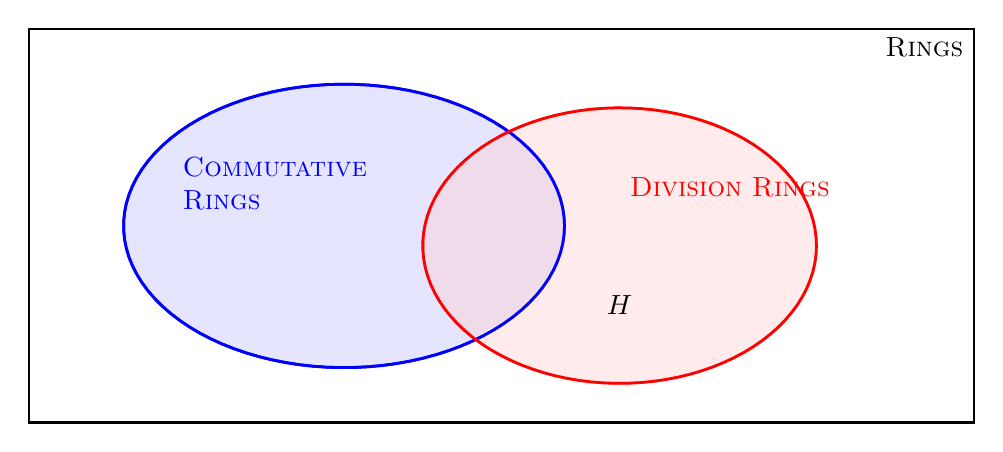
\begin{tikzpicture}[line width = 1]
\draw (0,0) rectangle (12,5);
\begin{scope}[shift={(4,2.5)}]
\fill[domain = 0:360,draw = blue, fill = blue!10, samples = 100] plot ({2.8*cos(\x)},{1.8*sin(\x)});
\end{scope}
\begin{scope}[shift={(7.5,2.25)}]
\fill[domain = 0:360,draw = red,fill = red!20, samples = 100,opacity=0.4] plot ({2.5*cos(\x)},{1.75*sin(\x)});
\end{scope}
\begin{scope}[shift={(4,2.5)}]
\draw[domain = 0:360,draw = blue, samples = 100,] plot ({2.8*cos(\x)},{1.8*sin(\x)});
\end{scope}
\begin{scope}[shift={(7.5,2.25)}]
\draw[domain = 0:360,draw = red, samples = 100] plot ({2.5*cos(\x)},{1.75*sin(\x)});
\end{scope}
\node[black, anchor = 20] at (12,5) {\textsc{Rings}};
\node[blue, anchor = 20, text width = 1in, align = flush left] at (4.5,3.5) {\textsc{Commutative Rings}};
\node[red, anchor = 20, text width = 1in, align = flush right] at (9.6,3.25) {\textsc{Division Rings}};
\node at (7.5,1.5) {$\mathbb{H}$};
\end{tikzpicture}
\end{center}
\end{problem}

% % % % % % % % % % % % % % % % % % % % % % % % % % % % % % % % % % % % % % % % % % % %
% SUBSECTION
% % % % % % % % % % % % % % % % % % % % % % % % % % % % % % % % % % % % % % % % % % % %
\subsection{Units}

Unless $R$ is actually a division ring, not all elements of $R$ will have a multiplicative inverse. Let's explore those elements that \emph{do} have an inverse.

\begin{definition}
Let $R$ be a ring with unity containing at least two elements. Then, $u\in R$ is called a \textbf{unit} if $u$ has a multiplicative inverse. The set of all units in $R$ is denoted $U(R)$.
\end{definition}


\begin{problem}
For each of the following rings, find all of the units, i.e.~determine $U(R)$.
\begin{multicols}{2}
\begin{enumerate}
\item $\mathbb{Z}$
\item $\mathbb{Z}_{5}$
\item $\mathbb{R}$
\item $\mathbb{R}[x]$
\end{enumerate}
\end{multicols}
\end{problem}

\begin{problem}
Consider the ring $\mathbb{Z}_{20}$. Find all units of $\mathbb{Z}_{20}$ and also find all zero divisors. What do you notice?
\end{problem}

\begin{problem}
Let $n$ be a positive integer. Make a conjecture about $U(\mathbb{Z}_n)$ by filling in the blank:  $U(\mathbb{Z}_n) = \{a\in \mathbb{Z}_n\mid\text{ \fillInBlank{fill in the blank} }\}$. What evidence do you have?
\end{problem}

\begin{theorem}\label{thm.UnitIsNotZeroDivisor}
Let $R$ be a ring with unity containing at least two elements. If $u\in R$ is a unit, then $u$ is \emph{not} a zero divisor.
\end{theorem}

\begin{problem}
Either prove or disprove the \emph{converse} of Theorem~\ref{thm.UnitIsNotZeroDivisor}.
\end{problem}

\begin{theorem}\label{thm.UnitsFormGroup}
Let $R$ be a ring with unity containing at least two elements. Then $(U(R),\cdot)$ is a group.
\end{theorem}
\end{section}


% % % % % % % % % % % % % % % % % % % % % % % % % % % % % % % % % % % % % % % % % % % %
% % % % % % % % % % % % % % % % % % % % % % % % % % % % % % % % % % % % % % % % % % % %
% SECTION
% % % % % % % % % % % % % % % % % % % % % % % % % % % % % % % % % % % % % % % % % % % %
% % % % % % % % % % % % % % % % % % % % % % % % % % % % % % % % % % % % % % % % % % % %
\begin{section}{An aside: matrix rings}

Matrix rings are really the prototypical ring with unity. Although you may have only seen matrices with real entries, it turns out that we can do matrix arithmetic with other types of entries, e.g.~entries from $\mathbb{C}$ or $\mathbb{Z}$. In fact, the usual matrix addition and multiplication makes sense when the entries come from any ring.

\begin{definition}
Let $R$ be a ring and $n$ a positive integer. Then $M_{n}(R)$ denotes the set of all $n\times n$ matrices whose entries come from $R$. The structure $(M_{n}(R),+,\cdot)$ consists of the set $M_{n}(R)$ of all $n\times n$ matrices whose entries come from $R$, together with the operations of usual matrix addition and matrix multiplication. 
\end{definition}

\begin{problem}
Provide examples of matrices satisfying each of the following conditions.
\begin{multicols}{2}
\begin{enumerate}
\item $A\in M_{3}(\mathbb{C})$ but $A\notin M_{2}(\mathbb{R})$
\item $B\in M_{2}(\mathbb{H})$ but $B\notin M_{2}(\mathbb{C})$
\item $C\in M_{2}\left(\mathbb{Q}\left(\sqrt{5}\right)\right)$ but $C\notin M_{2}(\mathbb{Q})$
\item $D\in M_{2}\left(\mathbb{R}[x]\right)$ but $D\notin M_{2}(\mathbb{R})$
\end{enumerate}
\end{multicols}
\end{problem}

\begin{problem}
Verify that $M_{2}(\mathbb{Z})$ is closed under matrix multiplication.
\end{problem}

The next fact shows that $M_{n}(R)$ is a ring with unity (for each positive $n$). Afterward, we will explore some of the other ring properties we discussed above.

\begin{fact} Let $R$ be any ring. The following are true for $M_{n}(R)$.
\begin{itemize}
\item \textbf{Addition Laws:} Addition is associative and commutative. There is a unique additive identity, namely the matrix with all entries equal to $0$, and every matrix $A$ has a unique additive inverse, denoted $-A$.
\item \textbf{Multiplication Laws:} Multiplication is associative. There is a unique multiplicative identity, namely the matrix with $1$'s on the main diagonal and $0$'s everywhere else.
\item \textbf{Distributivity Laws:} For all $A,B,C \in M_{n}(R)$, $A(B+C) = AB+AC$ and $(B+C)A = BA + CA$.
\end{itemize}
\end{fact}

\begin{problem}
Is $M_{2}(\mathbb{R})$ commutative? Prove your answer.
\end{problem}

\begin{problem}
Does $M_{2}(\mathbb{R})$ have zero divisors? Prove your answer. 
\end{problem}

The collection of units in a matrix ring forms a group with respect to matrix multiplication by Theorem~\ref{thm.UnitsFormGroup}. It is a very important object and even has a special name.

\begin{definition}
Let $R$ be a ring and $n$ a positive integer. The \textbf{general linear group} over the ring $R$,  denoted $\operatorname{GL}_n(R)$, is the group of units in the ring $M_{n}(R)$.
\end{definition}

\begin{problem}
Show that $\begin{bmatrix} i & 3\\ 0& i\end{bmatrix}\in\operatorname{GL}_{2}(\mathbb{C})$ by finding a multiplicative inverse for it. Also, find two different matrices in $M_{2}(\mathbb{C})$ that are \emph{not} in  $\operatorname{GL}_{2}(\mathbb{C})$.
\end{problem}
\end{section}


% % % % % % % % % % % % % % % % % % % % % % % % % % % % % % % % % % % % % % % % % % % %
% % % % % % % % % % % % % % % % % % % % % % % % % % % % % % % % % % % % % % % % % % % %
% SECTION
% % % % % % % % % % % % % % % % % % % % % % % % % % % % % % % % % % % % % % % % % % % %
% % % % % % % % % % % % % % % % % % % % % % % % % % % % % % % % % % % % % % % % % % % %
\begin{section}{Polynomial rings}

%Let's introduce some important terminology for working with polynomials.
%
%\begin{definition}
%Let $F$ be a field, and let $p(x) = a_0 + a_1x + \cdots + a_nx^n$ be in $F[x]$ with $a_n \neq 0$. Then $n$ is called the \textbf{degree} of $p(x)$, denoted $\deg(p(x))$. In words, $\deg(p(x))$ is the highest power of $x$ in $p(x)$ with a nonzero coefficient. The degree of the zero polynomial is undefined.
%\end{definition}



\end{section}